%%%%%%%%%%%%%% RNNs

\subsection{Recurrent NNs and LSTM}
\begin{frame}{Recurrent neural networks (RNNs)}
\vspace{-3mm}
\begin{itemize}
\item A neural network architecture for processing \textbf{sequences}.
\item[-] Consider a sequence of vectors $(x_1, x_2, ..., x_T)$ with $x_t \in \mathbb{R}^D$
\end{itemize}
\begin{itemize}
% \item RNNs have a \textbf{hidden state} $h_t \in \mathbb{R}^H$ which keep information about all past inputs until time $t$.
\item[-] \textbf{At each time step}, standard RNNs update its \textbf{hidden state} $h_t \in \mathbb{R}^H$ as a function of the \textbf{new input} $x_t$ and the \textbf{previous hidden states} $h_{t-1}$:
\[
h_t = f(W x_t + R h_{t-1} + b)
\]
where
\begin{itemize}
\item[-] $f$ is an activation function (e.g. $\tanh$)
\item[-] $W \in \mathbb{R}^{H \times D}$ and $R  \in \mathbb{R}^{H \times H}$
 are weight matrices, and $b \in \mathbb{R}^H$ a bias vector. 
\end{itemize}
\end{itemize}
\begin{figure}
                        \centering
                        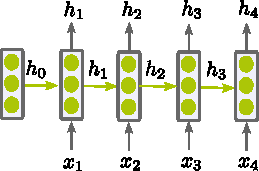
\includegraphics[width=.25\linewidth]{./figures/rnn.pdf}
\end{figure}
\begin{itemize}
\item Initial state $h_0$: typically chosen to be zero.
\item Compression of \textbf{variable length context} $x_1, ..., x_{t}$ to a fixed size vector $h_t$.
% \item We can also stack multiple such layers to make the model deeper.
\end{itemize}
\end{frame}


\begin{frame}{Recurrent neural networks (cont'd)}
\begin{itemize}
\item \textbf{Conceptually}: two inputs, two linear transformations, then sum the results.
\[
h_t = f(W x_t + R h_{t-1} + b)
\]
\item Equivalent but better for efficient computation: \textbf{concatenate} the inputs, do \textbf{one} ``big" linear transformation.
\[
h_t = f( [W, R] 
      \begin{bmatrix}
           x_t \\
           h_{t-1} \\
         \end{bmatrix}
 + b)
\]
where $[W R] \in \mathbb{R}^{H \times (D+H)}$ and
$ \begin{bmatrix} x_t \\ h_{t-1} \\ \end{bmatrix} \in \mathbb{R}^{(D+H) \times 1}$ 
\item Look at the equation: it is just like the standard feedforward layer but with the previous output as a part of the input: recurrent.
\item (You typically do not need to do this concatenation explicitly; PyTorch takes care of it internally)
\end{itemize}
\end{frame}


\begin{frame}{Recurrent neural networks, example}
\vspace{-5mm}
\textbf{Language modeling}:
\vsp
\begin{itemize}
\item \textbf{Task}: given a word sequence $w_0, ..., w_{i-1}$, predict the next word $w_i$.
\item \textbf{input} to the network at each time step: previous word $w_{i-1} \in V$, where $V$ is the vocabulary.
\item \textbf{output}: probability distribution over the vocabulary $w \in V$: $p(w | w_0^{i-1})$.\\ (normalized vector of size $|V|$). NB: notation $w_0^{i-1} = (w_0, ..., w_{i-1})$
\item[-] RNN state $h_{i-1}$ compactly represents  all previous words $w_0^{i-1}$.
\item[-] Step-by-step computation:
\end{itemize}
\begin{figure}
                        \centering
                        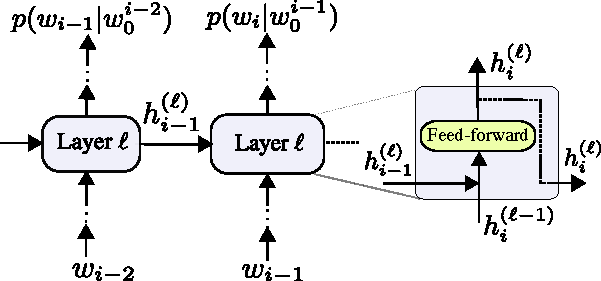
\includegraphics[width=.65\linewidth]{./figures/rnn_lm.pdf}
\end{figure}
%\end{minipage}
\end{frame}

\begin{frame}{Embedding layer}
\vspace{-5mm}
\begin{itemize}
\item Neural networks process \textbf{vectors}.
\item Discrete input symbols (e.g. words) can be represented by \emphbf{one-hot} vectors.
\begin{itemize}
\item[-] The size of a one-hot vector is the vocabulary size.
\item[-] An ID is given to each word.
\item[-] One hot vector's entries are all 0 except at the position corresponding to its ID where it's 1.
\end{itemize}

\end{itemize}
\begin{figure}
\centering
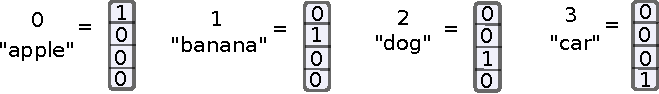
\includegraphics[width=.7\linewidth]{./figures/emb.pdf}
\end{figure}
\vsp
\begin{itemize}
\item Matrix multiplication with a one-hot vector is a (column) \textbf{look-up} operation (try to write it down!).
\item[-] No need to do the actual multiplication. 
\item \emphbf{Embedding layer}: input = discrete ID, output: its vector representation (trainable parameters).
\item[-] Learning of the continuous representation (vector) of discrete tokens is part of the model.
\item[-] In PyTorch: \codeb{nn.Embedding}
\end{itemize}
\end{frame}


\begin{frame}{Recurrent neural networks, training}
\begin{itemize}
\item The most popular training algorithm: back-propagation \textit{through time}.
\item By unfolding the recurrence, we obtain a deep feed-forward neural network (see how many layers
are between $x_1$ and $h_4$ in the figure)
\item[-] You can apply back-propagation to the resulting network.
\item[-] One update of parameters given a sequence (a batch of sequences).
\end{itemize}
\begin{figure}
\centering
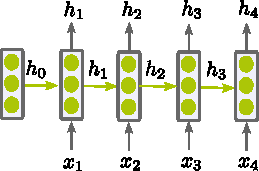
\includegraphics[width=.3\linewidth]{./figures/rnn.pdf}
\end{figure}
\vsp
\begin{itemize}
\item Unfolded model is as deep as the number of time steps. Typical problems:
\begin{itemize}
\item Exploding gradient
\item Vanishing gradient
\end{itemize}
\item Exploding gradient can be alleviated by \textit{clipping} gradient at some threshold (a hyper-parameter).
\end{itemize}

%\vsp
%Simple illustration by replacing $R$ by a scalar $0<\alpha<1$:\\
%\begin{itemize}
%\item[-] For each time step: the gradients are multiplied by $0<\alpha<1$. \\ $\rightarrow \alpha^2, \alpha^3,...$ get smaller (vanishing).\\
%\item[-] If $\alpha>1$, it gets larger (exploding).
%\item[-] Similar effect with matrices: having many matrix multiplications could attenuate gradients.
%\item[-] Exploding gradient can be alleviated by \textit{clipping} gradient at some threshold (hyper-parameter).
%\end{itemize}
\end{frame}

\begin{frame}[fragile]{Training, Batch, Padding}
\vspace{-5mm}
\begin{itemize}
\item How to create mini-batches to train RNNs?
\item Batch of shape e.g. (sequence length, batch size , feature dimension)
\item Sequences can have \emphbf{variable lengths}!
\end{itemize}
\vsp
We need to introduce \emphbf{padding}:
\begin{figure}
                        \centering
                        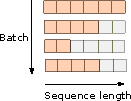
\includegraphics[width=.3\linewidth]{./figures/padding.pdf}
\end{figure}

\begin{itemize}
\item Add \textit{padding tokens} for short sequences such that all sequences get the same length (gray boxes above).
\item Run the RNN on the padded batch.
\item \textbf{Exclude the loss values from the padded positions}.\\
See for example \codeb{ignore\_index} argument in \codeb{nn.CrossEntropyLoss}.
\end{itemize}
\end{frame}

\begin{frame}{Truncated back-propagation through time}

\begin{itemize}
\item In some cases, sequences are too long for back-propagation through the entire sequence.
%\item In some cases, we would want to train RNNs to be evaluated/used for unlimited number of steps.
\item We typically use \emphbf{truncated} back-propagation through time.
%\item More we pad, more we waste computation...
%\item Trade-off: we can engineer it (e.g. sort sequences by lengths) but can lose model performance. 
%\item Or, if the nature of the problem allows it:
\begin{itemize}
\item Create fixed-length chunk/segments from the original sequences
by splitting/concatenating them.
\item \textbf{Carry over} the state vectors between two consecutive batches in the forward pass, but
\item Only propagate gradients \textbf{within} the batch in the backward pass.
\end{itemize}
\end{itemize}
% \vsp
\begin{figure}
                        \centering
                        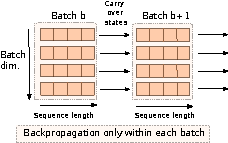
\includegraphics[width=.5\linewidth]{./figures/truncated_bptt.pdf}
\end{figure}


\end{frame}


\begin{frame}{Other architectures, long short-term memory (LSTM) and gating}
\begin{minipage}{0.6\linewidth}
\vsp
Now look at this RNN:
\begin{itemize}
\item Three gates, input/forget/output gates (parameterized by an NN):
\vspace{-3mm}
    \begin{eqnarray*} 
    i_{t} &=& \sigma(W_{i} x_{t} + R_{i} h_{t-1} + b_i) \\
    f_{t} &=& \sigma(W_{f} x_{t} + R_{f} h_{t-1} + b_f) \\
    o_t &=& \sigma(W_{o} x_{t} + R_{o} h_{t-1} + b_o) 
    \end{eqnarray*}
\item Input candidate:
\vspace{-3mm}
    \begin{eqnarray*} 
    z_t &=&  \tanh(W_{z} x_{t} + R_{z} h_{t-1} + b_z) 
    \end{eqnarray*}
\item Update cell states using the input and forget gates:
\vspace{-3mm}
    \begin{eqnarray*} 
    c_{t} &=&  f_{t} \odot c_{t-1} + i_{t} \odot  z_t 
    \end{eqnarray*}
\item Output: $h_t = o_{t} \odot \tanh(c_t)$
%\vspace{-3mm}
%    \begin{eqnarray*} 
%    h_t &=& o_{t} \odot \tanh(c_t)
%    \end{eqnarray*}
\end{itemize}
\vsp
(layer index $(\ell)$ omitted in the equations.)
\end{minipage}
\begin{minipage}{0.39\linewidth}
\begin{figure}
                        \centering
                        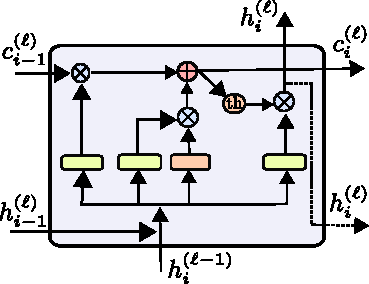
\includegraphics[width=.9\linewidth]{./figures/lstm.pdf}
\end{figure}
\end{minipage}
\end{frame}


\begin{frame}{Long short-term memory and gating (cont'd)}
\begin{minipage}{0.55\linewidth}
Special RNN architecture to alleviate vanishing gradient \citem{hochreiter1997long, gers2000learning}.
\begin{itemize}
\item two hidden state vectors
\item internal cell state with an additive connection over time (no multiplication with a weight matrix! good gradient flow).
\item \textbf{differentiable/soft multiplicative gates} (input/forget/output gates) control information flow around the cell
\item each gate parameterized by a neural network.
\end{itemize}
Inspired many other new architectures!
\end{minipage}
\begin{minipage}{0.4\linewidth}
\begin{figure}
                        \centering
                        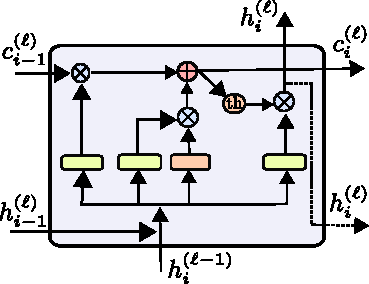
\includegraphics[width=.9\linewidth]{./figures/lstm.pdf}
\end{figure}
\end{minipage}
\end{frame}
%
%\begin{frame}{Long short-term memory and gating}
%\begin{minipage}{0.6\linewidth}
%\vsp
%\begin{itemize}
%\item Three gates (parameterized by NN):
%\vspace{-3mm}
%    \begin{eqnarray*} 
%    i_{t} &=& \sigma(W_{i} x_{t} + R_{i} h_{t-1} + b_i) \\
%    f_{t} &=& \sigma(W_{f} x_{t} + R_{f} h_{t-1} + b_f) \\
%    o_t &=& \sigma(W_{o} x_{t} + R_{o} h_{t-1} + b_o) 
%    \end{eqnarray*}
%\item Input candidate:
%\vspace{-3mm}
%    \begin{eqnarray*} 
%    z_t &=&  \tanh(W_{z} x_{t} + R_{z} h_{t-1} + b_z) 
%    \end{eqnarray*}
%\item Update cell states using input and forget gates:
%\vspace{-3mm}
%    \begin{eqnarray*} 
%    c_{t} &=&  f_{t} \odot c_{t-1} + i_{t} \odot  z_t 
%    \end{eqnarray*}
%\item Output: $h_t = o_{t} \odot \tanh(c_t)$
%%\vspace{-3mm}
%%    \begin{eqnarray*} 
%%    h_t &=& o_{t} \odot \tanh(c_t)
%%    \end{eqnarray*}
%\end{itemize}
%\vsp
%(layer index $(\ell)$ omitted in the equations.)
%\end{minipage}
%\begin{minipage}{0.39\linewidth}
%\begin{figure}
%                        \centering
%                        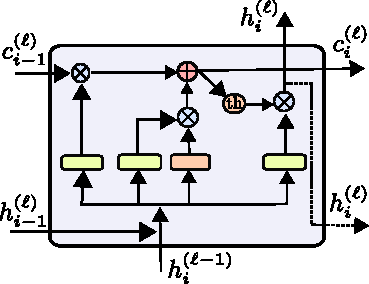
\includegraphics[width=.9\linewidth]{./figures/lstm.pdf}
%\end{figure}
%\end{minipage}
%\end{frame}

\begin{frame}{Long short-term memory and gating\\ (cont'd)}
\begin{itemize}
\item Again, linear transformations can be grouped.
\vspace{-3mm}
    \begin{eqnarray*}
      \begin{bmatrix}
           i_t \\
           f_t \\
           o_t \\
           z_t \\
         \end{bmatrix}
= 
      \begin{bmatrix}
           \sigma \\
           \sigma \\
           \sigma \\
           \tanh \\
         \end{bmatrix}
      \begin{bmatrix}
           W_{i}, R_{i} \\
           W_{f}, R_{f} \\
           W_{o}, R_{o} \\
           W_{z}, R_{z} \\
         \end{bmatrix} 
      \begin{bmatrix}
           x_t \\
           h_{t-1} \\
         \end{bmatrix}
+ 
      \begin{bmatrix}
           b_i \\
           b_f \\
           b_o \\
           b_z \\
         \end{bmatrix}
    \end{eqnarray*}
\item The rest as in the previous slide:
    \begin{eqnarray*}
    c_{t} &=&  f_{t} \odot c_{t-1} + i_{t} \odot  z_t \\
    h_t &=& o_{t} \odot \tanh(c_t)
    \end{eqnarray*}
%\vspace{-3mm}
%    \begin{eqnarray*}
%    h_t &=& o_{t} \odot \tanh(c_t)
%    \end{eqnarray*}
\end{itemize}
\vsp
NB: $      \begin{bmatrix}
           W_{i}, R_{i} \\
           W_{f}, R_{f} \\
           W_{o}, R_{o} \\
           W_{z}, R_{z} \\
         \end{bmatrix} \in \mathbb{R}^{4H \times (D+H)}$ and  
$\begin{bmatrix}
           b_i \\
           b_f \\
           b_o \\
           b_z \\
         \end{bmatrix} \in \mathbb{R}^{4H \times 1}$
\end{frame}



\begin{frame}{Recurrent neural networks, implementations}
\textbf{Two types} of RNN \emphbf{implementations}:
\begin{itemize}
\item \emphbf{Step-by-step} RNN functions:
\begin{itemize}
\item take one input, output one output.
\item expect you to write the loop over sequence. 
\item e.g. \codeb{torch.nn.LSTMCell}
\end{itemize}
\item \emphbf{Entire sequence} RNN functions:
\begin{itemize}
\item take sequence, output sequence
\item e.g. \codeb{torch.nn.LSTM}
\end{itemize}
\item In general: you should use the entire sequence one whenever you can,
which is optimized/faster.\\
\item[-] High-level spirit: use built-in code as much as possible (avoid your own plain code in Python).\\
% \item Some simple optimization possible (without C++) using TorchScript?
\end{itemize}
\end{frame}

\begin{frame}[fragile]{Recurrent neural networks, implementations (cont'd)}
Sequence-level function:
\begin{python}
>>> rnn = nn.LSTM(10, 20, 2)  # in_dim, out_dim, num_layers
>>> inputs = torch.randn(6, 3, 10)  # (len, B, in_dim)
>>> h0 = torch.randn(2, 3, 20)  # (num_layers, B, out_dim)
>>> c0 = torch.randn(2, 3, 20)  # (num_layers, B, out_dim)
# outputs of shape (len, B, out_dim)
>>> outputs, (hn, cn) = rnn(inputs, (h0, c0))
>>> outputs.size()
torch.Size([6, 3, 20])
\end{python}
NB:
\begin{itemize}
\item Only possible if all inputs are known (for example in training, or in some evaluation setups).
\item If the input also depends on the previous time steps (for example during \textit{search}; we will see later)
we have no other choice but to go step by step.
\end{itemize}
\end{frame}

\begin{frame}[fragile]{Recurrent neural networks, implementations (cont'd)}
Step-by-step function:
\begin{python}
>>> rnn = nn.LSTMCell(10, 20)  # in_dim, out_dim
>>> input = torch.randn(6, 3, 10)  # (len, B, in_dim)
>>> h = torch.randn(3, 20)  # (B, out_dim)
>>> c = torch.randn(3, 20)  # (B, out_dim)
>>> output = []
>>> for i in range(6):  # "manual" Python loop
        h, c = rnn(input[i], (h, c))
        output.append(h)
>>> output = torch.stack(output, 0)  # from list to tensor
>>> output.size()
torch.Size([6, 3, 20])
\end{python}
\end{frame}


\begin{frame}[fragile]{Example toy task: $N$-back}
Task:
\begin{itemize}
\item Input: sequence of numbers (between 0 and $k-1$).
\item Target at each position: 1 if the current input is equal
to the number at the $n$-th position back. 0 otherwise.
\item Sequences can have different lengths.
\end{itemize}
\vsp
\begin{figure}
                        \centering
                        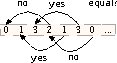
\includegraphics[width=.4\linewidth]{./figures/nback.pdf}
\end{figure}
\end{frame}

\begin{frame}[fragile]{Example toy task: $N$-back, model}
It is a binary classification at each position over a sequence.\\
Model:
\begin{itemize}
\item Read the input sequences using RNN.
\item Input: number between 0 and $k$ $\rightarrow$ discrete!
\item Actual input to the model: one hot representation: vector of size $k$
with zero entry everywhere except the position (embedding layer is not needed though: $k$ is small)
\item A classifier linear layer which maps the RNN's hidden vector to the
two output nodes (2 classes here; strictly speaking, one node is enough).
\item Cross entropy loss for training.
\end{itemize}
\end{frame}

%\begin{frame}[fragile]{Padding}
%
%\begin{itemize}
%\item The sequences can have different lengths!
%\end{itemize}
%\vsp
%We need to introduce \emphbf{padding}:
%\begin{itemize}
%\item How to construct batches with sequences of variable lengths?
%\item Add padding tokens (-1 for example) for short sequences such that
%all sequences get the same length.
%\item Run the RNN over the batch, and exclude padded positions from the loss computation.
%\item Note: more we pad, more we waste computation...
%\end{itemize}
%\end{frame}

\begin{frame}[fragile]{$N$-back, data generation}
\begin{itemize}
\item A helper function first:
\end{itemize}
\begin{python}
def nback(n, k, length, random_state):
  xi = random_state.randint(k, size=length)
  yi = np.zeros(length, dtype=int)

  for t in range(n, length):
    yi[t] = (xi[t-n] == xi[t])

  return xi, yi
\end{python}

\end{frame}

\begin{frame}[fragile]{$N$-back, data generation (cont'd)}
\vspace{-5mm}
\begin{itemize}
\item Main data generator:
\end{itemize}
\begin{python}
def create_dataset_nback(n_sequences, mean_length, std_length,
                         n, k, random_state):
  X, Y, lengths = [], [], []
  for _ in range(n_sequences):
    length = random_state.normal(loc=mean_length, scale=std_length)
    length = int(max(n+1, length))
    xi, yi = nback(n, k, length, random_state)
    X.append(xi)
    Y.append(yi)
    lengths.append(length)
  max_len = max(lengths)

  # We pad X w/ 0 (for one-hot), and Y w/ -1 (CE loss).
  X_arr = np.zeros((n_sequences, max_len), dtype=np.int64)
  Y_arr = np.zeros((n_sequences, max_len), dtype=np.int64) - 1

  for i in range(n_sequences):
    X_arr[i, 0: lengths[i]] = X[i]
    Y_arr[i, 0: lengths[i]] = Y[i]

  return X_arr, Y_arr, lengths
\end{python}

\end{frame}

\begin{frame}[fragile]{$N$-back, data generation (cont'd)}
\begin{itemize}
\item Generate data:
\end{itemize}
\begin{python}
import numpy as np

seed = 0
n = 3
k = 4
mean_length = 20
std_length = 5
n_sequences = 1000

random_state = np.random.RandomState(seed=seed)

X_train, Y_train, length_train = create_dataset_nback(
    n_sequences, mean_length, std_length, n, k, random_state)

X_val, Y_val, length_val = create_dataset_nback(
    n_sequences, mean_length, std_length, n, k, random_state)
\end{python}

\end{frame}

\begin{frame}[fragile]{$N$-back, RNN model}
\begin{itemize}
\item Create model: an RNN + a linear classifier layer.
\end{itemize}
\begin{python}
import torch.nn as nn

input_dim = 4
hidden_size = 64
num_layers = 1
num_classes = 2

rnn = nn.RNN(input_dim, hidden_size, num_layers)
linear = nn.Linear(hidden_size, num_classes)
h0 = torch.zeros(num_layers, n_sequences, hidden_size)  # init state
\end{python}

\begin{python}
import torch.optim as optim
# Again: alternatively write a model class!
params = list(rnn.parameters()) + list(linear.parameters())
optimizer = optim.Adam(params, lr=0.01)

# Exclude padded position (position with -1).
loss_fn = nn.CrossEntropyLoss(ignore_index=-1)
\end{python}
% loss_fn = nn.CrossEntropyLoss(ignore_index=-1, size_average=True) 
\end{frame}

\begin{frame}[fragile]{$N$-back, prepare data}
\begin{itemize}
\item Prepare data in the form/shape expected by RNNs:
\end{itemize}
\begin{python}
# prepare data
X = torch.from_numpy(X_train)
X = torch.nn.functional.one_hot(X)  # (B, len, k)
X = X.transpose(0, 1) 
X = X.float()

y = torch.from_numpy(Y_train)
y = y.transpose(0, 1).flatten()

# same for val:
X_val = torch.from_numpy(X_val)
X_val = torch.nn.functional.one_hot(X_val)
X_val = X_val.transpose(0, 1).float()
y_val = torch.from_numpy(Y_val).transpose(0, 1).flatten()
\end{python}

\end{frame}


\begin{frame}[fragile]{$N$-back, training}
\vspace{-5mm}
\begin{python}
num_train_steps = 200

total_val = sum(length_val)
total_tr = sum(length_train)

for step in range(num_train_steps):
  # more convenient if you had defined a model!
  # Please fix this in the exercise 6!
  rnn.train()
  linear.train()

  optimizer.zero_grad()
  output, hn = rnn(X, h0)
  output = output.view(-1, hidden_size)  # (B*len, dim)
  output = linear(output)

  loss = loss_fn(output, y)
  print(f"training loss: {loss}")

  loss.backward()
  optimizer.step()

# ... continue to the next slide ...

\end{python}

\end{frame}

\begin{frame}[fragile]{$N$-back, training (cont'd)}
\vspace{-5mm}
\begin{python}
# ... continue from the previous slide ...
  rnn.eval()
  linear.eval()  # more convenient if you had defined a model!
  with torch.no_grad():
    # Here evaluate also on training set (exercise 6).

    output_val, hn_val = rnn(X_val, h0)
    output_val = output_val.view(-1, hidden_size)
    output_val = linear(output_val)

    _, predicted_val = outputs_val.max(dim=1)
    correct_val = (predicted_val == y_val)

    # Important: do not count padded position!!
    mask_val = (y_val >= 0)
    correct_val = (correct_val * mask_val).sum().item()

    print(f'epoch: {step}, val acc: {100 * correct_val / total_val}')
\end{python}
\end{frame}


%\begin{frame}[fragile]{$N$-back, training (cont'd)}
%\vspace{-5mm}
%\begin{python}
%# ... continue from the previous slide ...
%  rnn.eval()
%  linear.eval()  # more convenient if you had defined a model!
%  with torch.no_grad():
%    output_tr, hn_tr = rnn(X, h0)
%    output_tr = output_tr.view(-1, hidden_size)
%    output_tr = linear(output_tr)
%    _, predicted_tr = outputs_tr.max(dim=1)
%    correct_tr = (predicted_tr == y)
%    mask_tr = (y >= 0)  # Important: do not count padded position!!
%    correct_tr = (correct_tr * mask_tr).sum().item()
%    print(f'epoch: {step}, train acc: {100 * correct_tr / total_tr}')
%
%    output_val, hn_val = rnn(X_val, h0)
%    output_val = output_val.view(-1, hidden_size)
%    output_val = linear(output_val)
%    _, predicted_val = outputs_val.max(dim=1)
%    correct_val = (predicted_val == y_val)
%    mask_val = (y_val >= 0)
%    correct_val = (correct_val * mask_val).sum().item()
%    print(f'epoch: {step}, val acc: {100 * correct_val / total_val}')
%\end{python}
%
%\end{frame}


\begin{frame}{Preview:\\ Exercise 6 \& Exercise 7 / Assignment 3}
	Both \emphbf{Exercise 6} and \emphbf{Exercise 7 / Assignment 3}
	\begin{itemize}
		\item Introduction to language modeling with RNNs
	\end{itemize}
\end{frame}

\begin{frame}{Preliminaries for Assignment 3,\\ Reminders}
\begin{minipage}{0.6\linewidth}
\begin{itemize}
\item Language models compute $p(w_i | w_0^{i-1})$ Notation: $w_0^{i-1} = (w_0, w_1, ..., w_{i-2}, w_{i-1})$
\item Given a sentence $w_1^N$,\\
$\displaystyle p(w_1, ..., w_N) = \prod_{i=1}^{N} p(w_i | w_0^{i-1})$
where\\ $w_0$ denotes an artificial start symbol
\item This can be used to compute probabilities of sentences,
e.g., which sentence should get a higher probability?
\begin{itemize}
\item[-] $p(\text{I hate cars \texttt{<eos>}})$
\item[-] $p(\text{I ate cars \texttt{<eos>}})$
\end{itemize}
where \texttt{<eos>} is the end-of-sentence token.
\item Another application in this assignment: text completion/generation.
\end{itemize}
\end{minipage}
\begin{minipage}{0.35\linewidth}
\begin{figure}
\centering
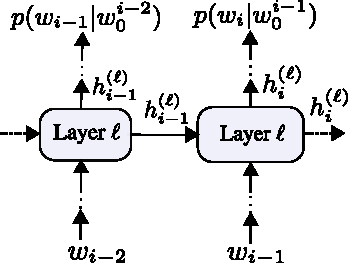
\includegraphics[width=1.\linewidth]{./figures/lm.pdf}
\end{figure}
\end{minipage}
\end{frame}

\begin{frame}{Preliminaries for Assignment 3}
\begin{itemize}
\item This \textbf{assignment}: text generation/completion.\\
\item[-] Once the model is trained, you will provide a beginning of some text $w_0^{i-1}$.
\item[-] You let the model complete your text.\\
You: \texttt{Dogs like best to}\\
Your LM: \texttt{eat , play , and sleep}
\end{itemize}
\vsp
\pause
How can this be done?
\pause
\begin{itemize}
\item Given the beginning of a sentence $w_0^{n-1}$,
let your LM compute $p(. | w_0^{n-1})$ (i.e., the probability distribution over the \textbf{next} word/token)
\item Then there are 2 possibilities:
\item[-] (1) Take the word with the highest probability. $\hat{w} = \argmax_w p(w | w_0^{n-1})$
\item[-] (2) Randomly sample $\hat{w}$ from the distribution $p(w | w_0^{n-1})$
\item Then feed the chosen word $\hat{w}$ to the LM as an input, and continue for a fixed number of steps.
\end{itemize}
\end{frame}

\begin{frame}{Preliminaries for Assignment 3,\\
Sampling vs. Search.}
\begin{itemize}
\item \emphbf{Search}: we want to find the most likely output from the model.
\item[-] In the assignment, \textbf{greedy search}:
\begin{itemize}
\item At each time step, obtain the most likely token.
\end{itemize}
\item \emphbf{Sampling}: we want to generate diverse outputs from the model.
\begin{itemize}
\item Randomly sample according to the model's output distribution.
\end{itemize}
In both cases, use the corresponding model output token as the input to the model for the next time step.
\end{itemize}
\end{frame}

\begin{frame}{Preliminaries for Assignment 3,\\
Pre-processing/Tokenization}
The data is a plain text file.
\begin{itemize}
\item The modeling unit must be defined: the text must be \textbf{tokenized}, e.g.
\item[-] Word level: i.e. split the text by white space.
\item[-] Character level
\end{itemize}
\vsp
Side note (not needed for A3): in general, depending on the task,
we also have to do some text pre-processing:
\begin{itemize}
\item[-] Normalization of lower/upper case, numbers, punctuations, or spelling, remove strings which are not really texts, etc.
\end{itemize}
\emphbf{Vocabulary} of the model:
\begin{itemize}
\item Add all characters found in the training set.
\item Add \textbf{special} tokens: pad token, unknown token, end-of-sentence token (not needed for A3), ...
\end{itemize}
See the helper code available on iCorsi.
\end{frame}
%
